% SOURCE: edit-harness/results/quant_survival/aggregate/gate_readout.json
% SOURCE FIELDS F5-A: cells.*.c3.{nf4dq,int8}.{r_func_mean,r_param_mean} (18 model/editor/layer/scheme aggregates).
% SOURCE FIELDS F5-B: cells.{Llama-3.2-1B_rome_L12,Llama-3.2-3B_rome_L24}.c3.nf4dq.F_above_mean.
% SOURCE FIELDS F5-C: cells.{Llama-3.2-1B_rome_L12,Qwen2.5-1.5B_rome_L21,Llama-3.2-3B_rome_L24}.{model,layer,c3.nf4dq.r_func_mean}.
% SCOPE F5-C/F5-D: one layer per model; depth is confounded with model; this is not a within-model depth profile.
% !TEX encoding = UTF-8 Unicode
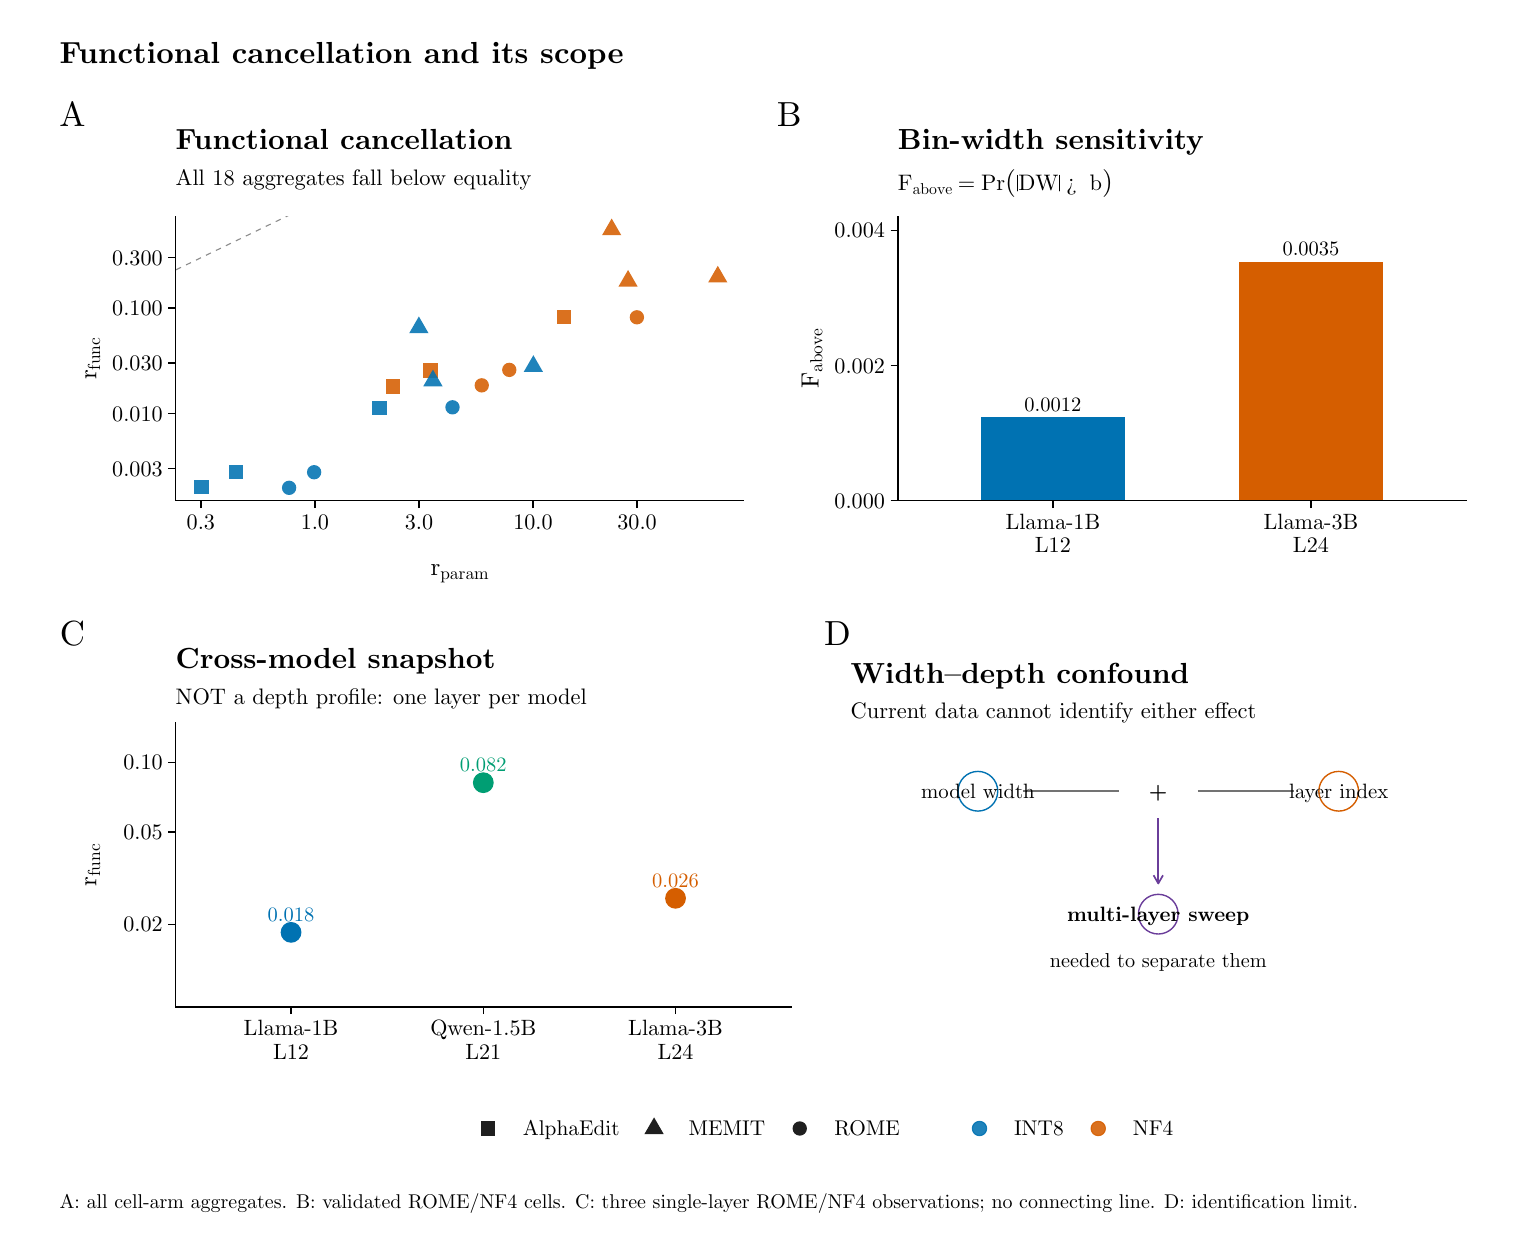
\begin{tikzpicture}[x=1pt,y=1pt]
\definecolor{fillColor}{RGB}{255,255,255}
\path[use as bounding box,fill=fillColor,fill opacity=0.00] (0,0) rectangle (531.18,433.62);
\begin{scope}
\path[clip] (  0.00,  0.00) rectangle (531.18,433.62);
\definecolor{drawColor}{RGB}{255,255,255}
\definecolor{fillColor}{RGB}{255,255,255}

\path[draw=drawColor,line width= 0.6pt,line join=round,line cap=round,fill=fillColor] (  0.00,  0.00) rectangle (531.18,433.62);
\end{scope}
\begin{scope}
\path[clip] (  5.50,225.42) rectangle (264.69,412.89);
\definecolor{drawColor}{RGB}{255,255,255}
\definecolor{fillColor}{RGB}{255,255,255}

\path[draw=drawColor,line width= 0.5pt,line join=round,line cap=round,fill=fillColor] (  5.50,225.42) rectangle (264.69,412.89);
\end{scope}
\begin{scope}
\path[clip] (264.69,225.42) rectangle (525.68,412.89);
\definecolor{drawColor}{RGB}{255,255,255}
\definecolor{fillColor}{RGB}{255,255,255}

\path[draw=drawColor,line width= 0.5pt,line join=round,line cap=round,fill=fillColor] (264.69,225.42) rectangle (525.68,412.89);
\end{scope}
\begin{scope}
\path[clip] ( 53.49,262.68) rectangle (258.69,365.28);
\definecolor{fillColor}{RGB}{255,255,255}

\path[fill=fillColor] ( 53.49,262.68) rectangle (258.69,365.28);
\definecolor{drawColor}{gray}{0.55}

\path[draw=drawColor,line width= 0.4pt,dash pattern=on 2pt off 2pt ,line join=round] (-151.70,246.97) -- (305.70,467.89);
\definecolor{fillColor}{RGB}{213,94,0}

\path[fill=fillColor,fill opacity=0.88] (211.02,364.65) --
	(214.51,358.61) --
	(207.54,358.61) --
	cycle;
\definecolor{fillColor}{RGB}{0,114,178}

\path[fill=fillColor,fill opacity=0.88] (141.36,329.26) --
	(144.84,323.22) --
	(137.87,323.22) --
	cycle;
\definecolor{fillColor}{RGB}{213,94,0}

\path[fill=fillColor,fill opacity=0.88] (129.43,301.42) --
	(134.61,301.42) --
	(134.61,306.60) --
	(129.43,306.60) --
	cycle;
\definecolor{fillColor}{RGB}{0,114,178}

\path[fill=fillColor,fill opacity=0.88] ( 60.23,265.03) --
	( 65.41,265.03) --
	( 65.41,270.21) --
	( 60.23,270.21) --
	cycle;
\definecolor{fillColor}{RGB}{213,94,0}

\path[fill=fillColor,fill opacity=0.88] (143.02,307.18) --
	(148.20,307.18) --
	(148.20,312.36) --
	(143.02,312.36) --
	cycle;
\definecolor{fillColor}{RGB}{0,114,178}

\path[fill=fillColor,fill opacity=0.88] ( 72.58,270.39) --
	( 77.76,270.39) --
	( 77.76,275.57) --
	( 72.58,275.57) --
	cycle;
\definecolor{fillColor}{RGB}{213,94,0}

\path[fill=fillColor,fill opacity=0.88] (249.37,347.57) --
	(252.85,341.54) --
	(245.88,341.54) --
	cycle;
\definecolor{fillColor}{RGB}{0,114,178}

\path[fill=fillColor,fill opacity=0.88] (182.73,315.26) --
	(186.21,309.22) --
	(179.24,309.22) --
	cycle;
\definecolor{fillColor}{RGB}{213,94,0}

\path[fill=fillColor,fill opacity=0.88] (191.18,326.41) --
	(196.36,326.41) --
	(196.36,331.59) --
	(191.18,331.59) --
	cycle;
\definecolor{fillColor}{RGB}{0,114,178}

\path[fill=fillColor,fill opacity=0.88] (124.55,293.61) --
	(129.73,293.61) --
	(129.73,298.79) --
	(124.55,298.79) --
	cycle;
\definecolor{fillColor}{RGB}{213,94,0}

\path[fill=fillColor,fill opacity=0.88] (216.95,346.06) --
	(220.43,340.02) --
	(213.46,340.02) --
	cycle;
\definecolor{fillColor}{RGB}{0,114,178}

\path[fill=fillColor,fill opacity=0.88] (146.44,310.07) --
	(149.93,304.03) --
	(142.95,304.03) --
	cycle;
\definecolor{fillColor}{RGB}{213,94,0}

\path[fill=fillColor,fill opacity=0.88] (164.08,304.37) circle (  2.59);
\definecolor{fillColor}{RGB}{0,114,178}

\path[fill=fillColor,fill opacity=0.88] ( 94.47,267.34) circle (  2.59);
\definecolor{fillColor}{RGB}{213,94,0}

\path[fill=fillColor,fill opacity=0.88] (174.03,309.96) circle (  2.59);
\definecolor{fillColor}{RGB}{0,114,178}

\path[fill=fillColor,fill opacity=0.88] (103.51,272.98) circle (  2.59);
\definecolor{fillColor}{RGB}{213,94,0}

\path[fill=fillColor,fill opacity=0.88] (220.14,328.96) circle (  2.59);
\definecolor{fillColor}{RGB}{0,114,178}

\path[fill=fillColor,fill opacity=0.88] (153.51,296.44) circle (  2.59);
\end{scope}
\begin{scope}
\path[clip] (  0.00,  0.00) rectangle (531.18,433.62);
\definecolor{drawColor}{RGB}{0,0,0}

\path[draw=drawColor,line width= 0.5pt,line join=round,line cap=rect] ( 53.49,262.68) --
	( 53.49,365.28);
\end{scope}
\begin{scope}
\path[clip] (  0.00,  0.00) rectangle (531.18,433.62);
\definecolor{drawColor}{RGB}{0,0,0}

\node[text=drawColor,anchor=base east,inner sep=0pt, outer sep=0pt, scale=  0.80] at ( 48.77,271.57) {0.003};

\node[text=drawColor,anchor=base east,inner sep=0pt, outer sep=0pt, scale=  0.80] at ( 48.77,291.47) {0.010};

\node[text=drawColor,anchor=base east,inner sep=0pt, outer sep=0pt, scale=  0.80] at ( 48.77,309.64) {0.030};

\node[text=drawColor,anchor=base east,inner sep=0pt, outer sep=0pt, scale=  0.80] at ( 48.77,329.54) {0.100};

\node[text=drawColor,anchor=base east,inner sep=0pt, outer sep=0pt, scale=  0.80] at ( 48.77,347.71) {0.300};
\end{scope}
\begin{scope}
\path[clip] (  0.00,  0.00) rectangle (531.18,433.62);
\definecolor{drawColor}{RGB}{0,0,0}

\path[draw=drawColor,line width= 0.5pt,line join=round] ( 50.87,274.32) --
	( 53.49,274.32);

\path[draw=drawColor,line width= 0.5pt,line join=round] ( 50.87,294.23) --
	( 53.49,294.23);

\path[draw=drawColor,line width= 0.5pt,line join=round] ( 50.87,312.39) --
	( 53.49,312.39);

\path[draw=drawColor,line width= 0.5pt,line join=round] ( 50.87,332.30) --
	( 53.49,332.30);

\path[draw=drawColor,line width= 0.5pt,line join=round] ( 50.87,350.46) --
	( 53.49,350.46);
\end{scope}
\begin{scope}
\path[clip] (  0.00,  0.00) rectangle (531.18,433.62);
\definecolor{drawColor}{RGB}{0,0,0}

\path[draw=drawColor,line width= 0.5pt,line join=round,line cap=rect] ( 53.49,262.68) --
	(258.69,262.68);
\end{scope}
\begin{scope}
\path[clip] (  0.00,  0.00) rectangle (531.18,433.62);
\definecolor{drawColor}{RGB}{0,0,0}

\path[draw=drawColor,line width= 0.5pt,line join=round] ( 62.58,260.05) --
	( 62.58,262.68);

\path[draw=drawColor,line width= 0.5pt,line join=round] (103.79,260.05) --
	(103.79,262.68);

\path[draw=drawColor,line width= 0.5pt,line join=round] (141.39,260.05) --
	(141.39,262.68);

\path[draw=drawColor,line width= 0.5pt,line join=round] (182.61,260.05) --
	(182.61,262.68);

\path[draw=drawColor,line width= 0.5pt,line join=round] (220.21,260.05) --
	(220.21,262.68);
\end{scope}
\begin{scope}
\path[clip] (  0.00,  0.00) rectangle (531.18,433.62);
\definecolor{drawColor}{RGB}{0,0,0}

\node[text=drawColor,anchor=base,inner sep=0pt, outer sep=0pt, scale=  0.80] at ( 62.58,252.44) {0.3};

\node[text=drawColor,anchor=base,inner sep=0pt, outer sep=0pt, scale=  0.80] at (103.79,252.44) {1.0};

\node[text=drawColor,anchor=base,inner sep=0pt, outer sep=0pt, scale=  0.80] at (141.39,252.44) {3.0};

\node[text=drawColor,anchor=base,inner sep=0pt, outer sep=0pt, scale=  0.80] at (182.61,252.44) {10.0};

\node[text=drawColor,anchor=base,inner sep=0pt, outer sep=0pt, scale=  0.80] at (220.21,252.44) {30.0};
\end{scope}
\begin{scope}
\path[clip] (  0.00,  0.00) rectangle (531.18,433.62);
\definecolor{drawColor}{RGB}{0,0,0}

\node[text=drawColor,anchor=base west,inner sep=0pt, outer sep=0pt, scale=  0.90] at (145.58,235.75) {r};

\node[text=drawColor,anchor=base west,inner sep=0pt, outer sep=0pt, scale=  0.63] at (149.10,234.39) {p};

\node[text=drawColor,anchor=base west,inner sep=0pt, outer sep=0pt, scale=  0.63] at (152.60,234.39) {a};

\node[text=drawColor,anchor=base west,inner sep=0pt, outer sep=0pt, scale=  0.63] at (155.75,234.39) {r};

\node[text=drawColor,anchor=base west,inner sep=0pt, outer sep=0pt, scale=  0.63] at (158.21,234.39) {a};

\node[text=drawColor,anchor=base west,inner sep=0pt, outer sep=0pt, scale=  0.63] at (161.36,234.39) {m};
\end{scope}
\begin{scope}
\path[clip] (  0.00,  0.00) rectangle (531.18,433.62);
\definecolor{drawColor}{RGB}{0,0,0}

\node[text=drawColor,rotate= 90.00,anchor=base west,inner sep=0pt, outer sep=0pt, scale=  0.90] at ( 24.82,306.36) {r};

\node[text=drawColor,rotate= 90.00,anchor=base west,inner sep=0pt, outer sep=0pt, scale=  0.63] at ( 26.18,309.88) {f};

\node[text=drawColor,rotate= 90.00,anchor=base west,inner sep=0pt, outer sep=0pt, scale=  0.63] at ( 26.18,311.81) {u};

\node[text=drawColor,rotate= 90.00,anchor=base west,inner sep=0pt, outer sep=0pt, scale=  0.63] at ( 26.18,315.30) {n};

\node[text=drawColor,rotate= 90.00,anchor=base west,inner sep=0pt, outer sep=0pt, scale=  0.63] at ( 26.18,318.80) {c};
\end{scope}
\begin{scope}
\path[clip] (  0.00,  0.00) rectangle (531.18,433.62);
\definecolor{drawColor}{RGB}{0,0,0}

\node[text=drawColor,anchor=base west,inner sep=0pt, outer sep=0pt, scale=  0.81] at ( 53.49,376.65) {All 18 aggregates fall below equality};
\end{scope}
\begin{scope}
\path[clip] (  0.00,  0.00) rectangle (531.18,433.62);
\definecolor{drawColor}{RGB}{0,0,0}

\node[text=drawColor,anchor=base west,inner sep=0pt, outer sep=0pt, scale=  1.05] at ( 53.49,389.52) {\bfseries Functional cancellation};
\end{scope}
\begin{scope}
\path[clip] (  0.00,  0.00) rectangle (531.18,433.62);
\definecolor{drawColor}{RGB}{0,0,0}

\node[text=drawColor,anchor=base,inner sep=0pt, outer sep=0pt, scale=  1.26] at ( 16.22,397.99) {A};
\end{scope}
\begin{scope}
\path[clip] (314.49,262.68) rectangle (519.68,365.28);
\definecolor{fillColor}{RGB}{255,255,255}

\path[fill=fillColor] (314.49,262.68) rectangle (519.68,365.28);
\definecolor{fillColor}{RGB}{0,114,178}

\path[fill=fillColor] (344.33,262.68) rectangle (396.57,292.81);
\definecolor{fillColor}{RGB}{213,94,0}

\path[fill=fillColor] (437.61,262.68) rectangle (489.84,349.00);
\definecolor{drawColor}{RGB}{0,0,0}

\node[text=drawColor,anchor=base,inner sep=0pt, outer sep=0pt, scale=  0.74] at (370.45,295.10) {0.0012};

\node[text=drawColor,anchor=base,inner sep=0pt, outer sep=0pt, scale=  0.74] at (463.72,351.29) {0.0035};
\end{scope}
\begin{scope}
\path[clip] (  0.00,  0.00) rectangle (531.18,433.62);
\definecolor{drawColor}{RGB}{0,0,0}

\path[draw=drawColor,line width= 0.5pt,line join=round,line cap=rect] (314.49,262.68) --
	(314.49,365.28);
\end{scope}
\begin{scope}
\path[clip] (  0.00,  0.00) rectangle (531.18,433.62);
\definecolor{drawColor}{RGB}{0,0,0}

\node[text=drawColor,anchor=base east,inner sep=0pt, outer sep=0pt, scale=  0.80] at (309.76,259.92) {0.000};

\node[text=drawColor,anchor=base east,inner sep=0pt, outer sep=0pt, scale=  0.80] at (309.76,308.78) {0.002};

\node[text=drawColor,anchor=base east,inner sep=0pt, outer sep=0pt, scale=  0.80] at (309.76,357.64) {0.004};
\end{scope}
\begin{scope}
\path[clip] (  0.00,  0.00) rectangle (531.18,433.62);
\definecolor{drawColor}{RGB}{0,0,0}

\path[draw=drawColor,line width= 0.5pt,line join=round] (311.86,262.68) --
	(314.49,262.68);

\path[draw=drawColor,line width= 0.5pt,line join=round] (311.86,311.54) --
	(314.49,311.54);

\path[draw=drawColor,line width= 0.5pt,line join=round] (311.86,360.40) --
	(314.49,360.40);
\end{scope}
\begin{scope}
\path[clip] (  0.00,  0.00) rectangle (531.18,433.62);
\definecolor{drawColor}{RGB}{0,0,0}

\path[draw=drawColor,line width= 0.5pt,line join=round,line cap=rect] (314.49,262.68) --
	(519.68,262.68);
\end{scope}
\begin{scope}
\path[clip] (  0.00,  0.00) rectangle (531.18,433.62);
\definecolor{drawColor}{RGB}{0,0,0}

\path[draw=drawColor,line width= 0.5pt,line join=round] (370.45,260.05) --
	(370.45,262.68);

\path[draw=drawColor,line width= 0.5pt,line join=round] (463.72,260.05) --
	(463.72,262.68);
\end{scope}
\begin{scope}
\path[clip] (  0.00,  0.00) rectangle (531.18,433.62);
\definecolor{drawColor}{RGB}{0,0,0}

\node[text=drawColor,anchor=base,inner sep=0pt, outer sep=0pt, scale=  0.80] at (370.45,252.44) {Llama-1B};

\node[text=drawColor,anchor=base,inner sep=0pt, outer sep=0pt, scale=  0.80] at (370.45,243.80) {L12};

\node[text=drawColor,anchor=base,inner sep=0pt, outer sep=0pt, scale=  0.80] at (463.72,252.44) {Llama-3B};

\node[text=drawColor,anchor=base,inner sep=0pt, outer sep=0pt, scale=  0.80] at (463.72,243.80) {L24};
\end{scope}
\begin{scope}
\path[clip] (  0.00,  0.00) rectangle (531.18,433.62);
\definecolor{drawColor}{RGB}{0,0,0}

\node[text=drawColor,rotate= 90.00,anchor=base west,inner sep=0pt, outer sep=0pt, scale=  0.90] at (285.81,303.08) {F};

\node[text=drawColor,rotate= 90.00,anchor=base west,inner sep=0pt, outer sep=0pt, scale=  0.63] at (287.17,308.96) {a};

\node[text=drawColor,rotate= 90.00,anchor=base west,inner sep=0pt, outer sep=0pt, scale=  0.63] at (287.17,312.11) {b};

\node[text=drawColor,rotate= 90.00,anchor=base west,inner sep=0pt, outer sep=0pt, scale=  0.63] at (287.17,315.60) {o};

\node[text=drawColor,rotate= 90.00,anchor=base west,inner sep=0pt, outer sep=0pt, scale=  0.63] at (287.17,318.75) {v};

\node[text=drawColor,rotate= 90.00,anchor=base west,inner sep=0pt, outer sep=0pt, scale=  0.63] at (287.17,322.08) {e};
\end{scope}
\begin{scope}
\path[clip] (  0.00,  0.00) rectangle (531.18,433.62);
\definecolor{drawColor}{RGB}{0,0,0}

\node[text=drawColor,anchor=base west,inner sep=0pt, outer sep=0pt, scale=  0.81] at (314.49,374.64) {F};

\node[text=drawColor,anchor=base west,inner sep=0pt, outer sep=0pt, scale=  0.57] at (319.77,373.42) {a};

\node[text=drawColor,anchor=base west,inner sep=0pt, outer sep=0pt, scale=  0.57] at (322.61,373.42) {b};

\node[text=drawColor,anchor=base west,inner sep=0pt, outer sep=0pt, scale=  0.57] at (325.76,373.42) {o};

\node[text=drawColor,anchor=base west,inner sep=0pt, outer sep=0pt, scale=  0.57] at (328.59,373.42) {v};

\node[text=drawColor,anchor=base west,inner sep=0pt, outer sep=0pt, scale=  0.57] at (331.58,373.42) {e};

\node[text=drawColor,anchor=base west,inner sep=0pt, outer sep=0pt, scale=  0.81] at (336.16,374.64) {=};

\node[text=drawColor,anchor=base west,inner sep=0pt, outer sep=0pt, scale=  0.81] at (344.52,374.64) {Pr};

\node[text=drawColor,anchor=base west,inner sep=0pt, outer sep=0pt, scale=  1.01] at (353.21,374.64) {(};

\path[draw=drawColor,line width= 0.4pt,line join=round,line cap=round] (357.55,374.64) --
	(357.55,380.22);

\node[text=drawColor,anchor=base west,inner sep=0pt, outer sep=0pt, scale=  0.81] at (357.97,374.64) {D};

\node[text=drawColor,anchor=base west,inner sep=0pt, outer sep=0pt, scale=  0.81] at (364.15,374.64) {W};

\path[draw=drawColor,line width= 0.4pt,line join=round,line cap=round] (372.89,374.64) --
	(372.89,380.22);

\node[text=drawColor,anchor=base west,inner sep=0pt, outer sep=0pt, scale=  0.81] at (375.36,374.64) {>};

\node[text=drawColor,anchor=base west,inner sep=0pt, outer sep=0pt, scale=  0.81] at (383.72,374.64) {b};

\node[text=drawColor,anchor=base west,inner sep=0pt, outer sep=0pt, scale=  1.01] at (388.22,374.64) {)};
\end{scope}
\begin{scope}
\path[clip] (  0.00,  0.00) rectangle (531.18,433.62);
\definecolor{drawColor}{RGB}{0,0,0}

\node[text=drawColor,anchor=base west,inner sep=0pt, outer sep=0pt, scale=  1.05] at (314.49,389.52) {\bfseries Bin-width sensitivity};
\end{scope}
\begin{scope}
\path[clip] (  0.00,  0.00) rectangle (531.18,433.62);
\definecolor{drawColor}{RGB}{0,0,0}

\node[text=drawColor,anchor=base,inner sep=0pt, outer sep=0pt, scale=  1.26] at (275.15,397.99) {B};
\end{scope}
\begin{scope}
\path[clip] (  5.50, 17.36) rectangle (281.78,225.42);
\definecolor{drawColor}{RGB}{255,255,255}
\definecolor{fillColor}{RGB}{255,255,255}

\path[draw=drawColor,line width= 0.5pt,line join=round,line cap=round,fill=fillColor] (  5.50, 17.36) rectangle (281.78,225.42);
\end{scope}
\begin{scope}
\path[clip] (281.78, 17.36) rectangle (525.68,225.42);

\path[] (281.78, 17.36) rectangle (525.68,225.42);
\end{scope}
\begin{scope}
\path[clip] ( 53.49, 79.74) rectangle (275.78,182.35);
\definecolor{fillColor}{RGB}{255,255,255}

\path[fill=fillColor] ( 53.49, 79.74) rectangle (275.78,182.35);
\definecolor{drawColor}{RGB}{0,114,178}
\definecolor{fillColor}{RGB}{0,114,178}

\path[draw=drawColor,line width= 0.4pt,line join=round,line cap=round,fill=fillColor] ( 95.17,106.71) circle (  3.55);
\definecolor{drawColor}{RGB}{213,94,0}
\definecolor{fillColor}{RGB}{213,94,0}

\path[draw=drawColor,line width= 0.4pt,line join=round,line cap=round,fill=fillColor] (234.10,119.02) circle (  3.55);
\definecolor{drawColor}{RGB}{0,158,115}
\definecolor{fillColor}{RGB}{0,158,115}

\path[draw=drawColor,line width= 0.4pt,line join=round,line cap=round,fill=fillColor] (164.64,160.79) circle (  3.55);
\definecolor{drawColor}{RGB}{0,114,178}

\node[text=drawColor,anchor=base,inner sep=0pt, outer sep=0pt, scale=  0.74] at ( 95.17,110.79) {0.018};
\definecolor{drawColor}{RGB}{213,94,0}

\node[text=drawColor,anchor=base,inner sep=0pt, outer sep=0pt, scale=  0.74] at (234.10,123.09) {0.026};
\definecolor{drawColor}{RGB}{0,158,115}

\node[text=drawColor,anchor=base,inner sep=0pt, outer sep=0pt, scale=  0.74] at (164.64,164.87) {0.082};
\end{scope}
\begin{scope}
\path[clip] (  0.00,  0.00) rectangle (531.18,433.62);
\definecolor{drawColor}{RGB}{0,0,0}

\path[draw=drawColor,line width= 0.5pt,line join=round,line cap=rect] ( 53.49, 79.74) --
	( 53.49,182.35);
\end{scope}
\begin{scope}
\path[clip] (  0.00,  0.00) rectangle (531.18,433.62);
\definecolor{drawColor}{RGB}{0,0,0}

\node[text=drawColor,anchor=base east,inner sep=0pt, outer sep=0pt, scale=  0.80] at ( 48.77,106.86) {0.02};

\node[text=drawColor,anchor=base east,inner sep=0pt, outer sep=0pt, scale=  0.80] at ( 48.77,140.18) {0.05};

\node[text=drawColor,anchor=base east,inner sep=0pt, outer sep=0pt, scale=  0.80] at ( 48.77,165.39) {0.10};
\end{scope}
\begin{scope}
\path[clip] (  0.00,  0.00) rectangle (531.18,433.62);
\definecolor{drawColor}{RGB}{0,0,0}

\path[draw=drawColor,line width= 0.5pt,line join=round] ( 50.87,109.61) --
	( 53.49,109.61);

\path[draw=drawColor,line width= 0.5pt,line join=round] ( 50.87,142.94) --
	( 53.49,142.94);

\path[draw=drawColor,line width= 0.5pt,line join=round] ( 50.87,168.14) --
	( 53.49,168.14);
\end{scope}
\begin{scope}
\path[clip] (  0.00,  0.00) rectangle (531.18,433.62);
\definecolor{drawColor}{RGB}{0,0,0}

\path[draw=drawColor,line width= 0.5pt,line join=round,line cap=rect] ( 53.49, 79.74) --
	(275.78, 79.74);
\end{scope}
\begin{scope}
\path[clip] (  0.00,  0.00) rectangle (531.18,433.62);
\definecolor{drawColor}{RGB}{0,0,0}

\path[draw=drawColor,line width= 0.5pt,line join=round] ( 95.17, 77.12) --
	( 95.17, 79.74);

\path[draw=drawColor,line width= 0.5pt,line join=round] (164.64, 77.12) --
	(164.64, 79.74);

\path[draw=drawColor,line width= 0.5pt,line join=round] (234.10, 77.12) --
	(234.10, 79.74);
\end{scope}
\begin{scope}
\path[clip] (  0.00,  0.00) rectangle (531.18,433.62);
\definecolor{drawColor}{RGB}{0,0,0}

\node[text=drawColor,anchor=base,inner sep=0pt, outer sep=0pt, scale=  0.80] at ( 95.17, 69.51) {Llama-1B};

\node[text=drawColor,anchor=base,inner sep=0pt, outer sep=0pt, scale=  0.80] at ( 95.17, 60.87) {L12};

\node[text=drawColor,anchor=base,inner sep=0pt, outer sep=0pt, scale=  0.80] at (164.64, 69.51) {Qwen-1.5B};

\node[text=drawColor,anchor=base,inner sep=0pt, outer sep=0pt, scale=  0.80] at (164.64, 60.87) {L21};

\node[text=drawColor,anchor=base,inner sep=0pt, outer sep=0pt, scale=  0.80] at (234.10, 69.51) {Llama-3B};

\node[text=drawColor,anchor=base,inner sep=0pt, outer sep=0pt, scale=  0.80] at (234.10, 60.87) {L24};
\end{scope}
\begin{scope}
\path[clip] (  0.00,  0.00) rectangle (531.18,433.62);
\definecolor{drawColor}{RGB}{0,0,0}

\node[text=drawColor,rotate= 90.00,anchor=base west,inner sep=0pt, outer sep=0pt, scale=  0.90] at ( 24.82,123.42) {r};

\node[text=drawColor,rotate= 90.00,anchor=base west,inner sep=0pt, outer sep=0pt, scale=  0.63] at ( 26.18,126.95) {f};

\node[text=drawColor,rotate= 90.00,anchor=base west,inner sep=0pt, outer sep=0pt, scale=  0.63] at ( 26.18,128.87) {u};

\node[text=drawColor,rotate= 90.00,anchor=base west,inner sep=0pt, outer sep=0pt, scale=  0.63] at ( 26.18,132.37) {n};

\node[text=drawColor,rotate= 90.00,anchor=base west,inner sep=0pt, outer sep=0pt, scale=  0.63] at ( 26.18,135.87) {c};
\end{scope}
\begin{scope}
\path[clip] (  0.00,  0.00) rectangle (531.18,433.62);
\definecolor{drawColor}{RGB}{0,0,0}

\node[text=drawColor,anchor=base west,inner sep=0pt, outer sep=0pt, scale=  0.81] at ( 53.49,189.17) {NOT a depth profile: one layer per model};
\end{scope}
\begin{scope}
\path[clip] (  0.00,  0.00) rectangle (531.18,433.62);
\definecolor{drawColor}{RGB}{0,0,0}

\node[text=drawColor,anchor=base west,inner sep=0pt, outer sep=0pt, scale=  1.05] at ( 53.49,202.04) {\bfseries Cross-model snapshot};
\end{scope}
\begin{scope}
\path[clip] (  0.00,  0.00) rectangle (531.18,433.62);
\definecolor{drawColor}{RGB}{0,0,0}

\node[text=drawColor,anchor=base,inner sep=0pt, outer sep=0pt, scale=  1.26] at ( 16.22,210.51) {C};
\end{scope}
\begin{scope}
\path[clip] (  0.00,  0.00) rectangle (531.18,433.62);
\definecolor{drawColor}{gray}{0.45}

\path[draw=drawColor,line width= 0.6pt,line join=round] (359.65,157.70) -- (394.20,157.70);

\path[draw=drawColor,line width= 0.6pt,line join=round] (422.88,157.70) -- (457.43,157.70);
\definecolor{drawColor}{RGB}{106,61,154}

\path[draw=drawColor,line width= 0.6pt,line join=round] (408.54,147.93) -- (408.54,124.38);

\path[draw=drawColor,line width= 0.6pt,line join=round] (406.84,127.34) --
	(408.54,124.38) --
	(410.25,127.34);
\definecolor{drawColor}{RGB}{0,114,178}
\definecolor{fillColor}{RGB}{255,255,255}

\path[draw=drawColor,line width= 0.5pt,line join=round,line cap=round,fill=fillColor] (343.36,157.70) circle (  7.17);
\definecolor{drawColor}{RGB}{213,94,0}

\path[draw=drawColor,line width= 0.5pt,line join=round,line cap=round,fill=fillColor] (473.73,157.70) circle (  7.17);
\definecolor{drawColor}{RGB}{106,61,154}

\path[draw=drawColor,line width= 0.5pt,line join=round,line cap=round,fill=fillColor] (408.54,113.28) circle (  7.17);
\definecolor{drawColor}{RGB}{0,0,0}

\node[text=drawColor,anchor=base,inner sep=0pt, outer sep=0pt, scale=  0.75] at (343.36,155.10) {model width};

\node[text=drawColor,anchor=base,inner sep=0pt, outer sep=0pt, scale=  0.75] at (408.54,155.10) {\bfseries +};

\node[text=drawColor,anchor=base,inner sep=0pt, outer sep=0pt, scale=  0.75] at (473.73,155.10) {layer index};

\node[text=drawColor,anchor=base,inner sep=0pt, outer sep=0pt, scale=  0.75] at (408.54,110.68) {\bfseries multi-layer sweep};

\node[text=drawColor,anchor=base,inner sep=0pt, outer sep=0pt, scale=  0.73] at (408.54, 93.90) {needed to separate them};
\end{scope}
\begin{scope}
\path[clip] (  0.00,  0.00) rectangle (531.18,433.62);
\definecolor{drawColor}{RGB}{0,0,0}

\node[text=drawColor,anchor=base west,inner sep=0pt, outer sep=0pt, scale=  0.81] at (297.40,183.92) {Current data cannot identify either effect};
\end{scope}
\begin{scope}
\path[clip] (  0.00,  0.00) rectangle (531.18,433.62);
\definecolor{drawColor}{RGB}{0,0,0}

\node[text=drawColor,anchor=base west,inner sep=0pt, outer sep=0pt, scale=  1.05] at (297.40,196.79) {\bfseries Width--depth confound};
\end{scope}
\begin{scope}
\path[clip] (  0.00,  0.00) rectangle (531.18,433.62);
\definecolor{drawColor}{RGB}{0,0,0}

\node[text=drawColor,anchor=base,inner sep=0pt, outer sep=0pt, scale=  1.26] at (292.59,210.51) {D};
\end{scope}
\begin{scope}
\path[clip] (  0.00,  0.00) rectangle (531.18,433.62);
\definecolor{fillColor}{RGB}{255,255,255}

\path[fill=fillColor] (153.95, 23.36) rectangle (320.46, 48.31);
\end{scope}
\begin{scope}
\path[clip] (  0.00,  0.00) rectangle (531.18,433.62);
\definecolor{fillColor}{RGB}{255,255,255}

\path[fill=fillColor] (159.20, 28.61) rectangle (173.66, 43.06);
\definecolor{fillColor}{RGB}{0,0,0}

\path[fill=fillColor,fill opacity=0.88] (163.84, 33.25) --
	(169.02, 33.25) --
	(169.02, 38.42) --
	(163.84, 38.42) --
	cycle;
\end{scope}
\begin{scope}
\path[clip] (  0.00,  0.00) rectangle (531.18,433.62);
\definecolor{fillColor}{RGB}{255,255,255}

\path[fill=fillColor] (219.12, 28.61) rectangle (233.57, 43.06);
\definecolor{fillColor}{RGB}{0,0,0}

\path[fill=fillColor,fill opacity=0.88] (226.35, 39.86) --
	(229.83, 33.82) --
	(222.86, 33.82) --
	cycle;
\end{scope}
\begin{scope}
\path[clip] (  0.00,  0.00) rectangle (531.18,433.62);
\definecolor{fillColor}{RGB}{255,255,255}

\path[fill=fillColor] (271.77, 28.61) rectangle (286.22, 43.06);
\definecolor{fillColor}{RGB}{0,0,0}

\path[fill=fillColor,fill opacity=0.88] (278.99, 35.84) circle (  2.59);
\end{scope}
\begin{scope}
\path[clip] (  0.00,  0.00) rectangle (531.18,433.62);
\definecolor{drawColor}{RGB}{0,0,0}

\node[text=drawColor,anchor=base west,inner sep=0pt, outer sep=0pt, scale=  0.77] at (178.91, 33.18) {AlphaEdit};
\end{scope}
\begin{scope}
\path[clip] (  0.00,  0.00) rectangle (531.18,433.62);
\definecolor{drawColor}{RGB}{0,0,0}

\node[text=drawColor,anchor=base west,inner sep=0pt, outer sep=0pt, scale=  0.77] at (238.82, 33.18) {MEMIT};
\end{scope}
\begin{scope}
\path[clip] (  0.00,  0.00) rectangle (531.18,433.62);
\definecolor{drawColor}{RGB}{0,0,0}

\node[text=drawColor,anchor=base west,inner sep=0pt, outer sep=0pt, scale=  0.77] at (291.47, 33.18) {ROME};
\end{scope}
\begin{scope}
\path[clip] (  0.00,  0.00) rectangle (531.18,433.62);
\definecolor{fillColor}{RGB}{255,255,255}

\path[fill=fillColor] (331.46, 23.36) rectangle (419.23, 48.31);
\end{scope}
\begin{scope}
\path[clip] (  0.00,  0.00) rectangle (531.18,433.62);
\definecolor{fillColor}{RGB}{255,255,255}

\path[fill=fillColor] (336.71, 28.61) rectangle (351.16, 43.06);
\definecolor{drawColor}{RGB}{0,114,178}
\definecolor{fillColor}{RGB}{0,114,178}

\path[draw=drawColor,draw opacity=0.88,line width= 0.4pt,line join=round,line cap=round,fill=fillColor,fill opacity=0.88] (343.93, 35.84) circle (  2.59);
\end{scope}
\begin{scope}
\path[clip] (  0.00,  0.00) rectangle (531.18,433.62);
\definecolor{fillColor}{RGB}{255,255,255}

\path[fill=fillColor] (379.62, 28.61) rectangle (394.08, 43.06);
\definecolor{drawColor}{RGB}{213,94,0}
\definecolor{fillColor}{RGB}{213,94,0}

\path[draw=drawColor,draw opacity=0.88,line width= 0.4pt,line join=round,line cap=round,fill=fillColor,fill opacity=0.88] (386.85, 35.84) circle (  2.59);
\end{scope}
\begin{scope}
\path[clip] (  0.00,  0.00) rectangle (531.18,433.62);
\definecolor{drawColor}{RGB}{0,0,0}

\node[text=drawColor,anchor=base west,inner sep=0pt, outer sep=0pt, scale=  0.77] at (356.41, 33.18) {INT8};
\end{scope}
\begin{scope}
\path[clip] (  0.00,  0.00) rectangle (531.18,433.62);
\definecolor{drawColor}{RGB}{0,0,0}

\node[text=drawColor,anchor=base west,inner sep=0pt, outer sep=0pt, scale=  0.77] at (399.33, 33.18) {NF4};
\end{scope}
\begin{scope}
\path[clip] (  0.00,  0.00) rectangle (531.18,433.62);
\definecolor{drawColor}{RGB}{0,0,0}

\node[text=drawColor,anchor=base west,inner sep=0pt, outer sep=0pt, scale=  0.72] at ( 11.50,  6.90) {A: all cell-arm aggregates. B: validated ROME/NF4 cells. C: three single-layer ROME/NF4 observations; no connecting line. D: identification limit.};
\end{scope}
\begin{scope}
\path[clip] (  0.00,  0.00) rectangle (531.18,433.62);
\definecolor{drawColor}{RGB}{0,0,0}

\node[text=drawColor,anchor=base west,inner sep=0pt, outer sep=0pt, scale=  1.10] at ( 11.50,420.53) {\bfseries Functional cancellation and its scope};
\end{scope}
\end{tikzpicture}
